\documentclass[12pt]{article}

\usepackage[utf8x]{inputenc}

\usepackage[a4paper,top=3cm,bottom=2.5cm,left=2.5cm,right=3cm,marginparwidth=1.75cm]{geometry}
\usepackage[hidelinks]{hyperref}
%% Useful packages
\usepackage{graphicx}
\usepackage{array}
\usepackage{wrapfig}

\graphicspath{{./Images}}



\begin{document}
\begin{titlepage}

    \newcommand{\HRule}{\rule{\linewidth}{0.5mm}} 							% horizontal line and its thickness
    \center

    % University
    \textsc{\LARGE University of Moratuwa}\\[1cm]

    % Document info
    \textsc{\Large Electronics - III}\\[0.2cm]
    \textsc{\large EN2110}\\[1cm] 										% Course Code
    \HRule \\[0.8cm]
    { \huge \bfseries Proposal : MPPT CHARGER}\\[0.7cm]
    \HRule \\[2cm]
    \large
    \emph{\large Team : Trouble Makers}\\
    [0.3cm]
    \begin{tabular}{ l r }
        Tharindu.O.K.D      & 190622R \\
        Ranasighe.R.A.D.V.C & 190497K \\
        S.Sanjith           & 190562G \\
        Yasarathna D.D.K.B. & 190719V \\
    \end{tabular}\\
    [1.5cm]
    {\large \today}\\[2cm]
    
\includegraphics[width=0.4\textwidth]{mora.png}\\[1cm] 	% University logo
    \vfill
\end{titlepage}
\section*{Introduction}
We team "Trouble Makers" are proposing a design for the MPPT charge controller as our project idea for the EN2110 module. We hope to make a modular design with the fusion of both analog and digital domains to achieve maximum performance with power efficiency.  Our solution mainly focussed on bringing the solution into the low power applications by making the design cost-effective.
\section*{Description}
A charge controller is a device that controls the current drawn in or out of batteries to provide over-voltage protection.
There are two main approaches used for such a controller. One is the PWM controller which controls the voltage supply through pulse width modulation to maintain a constant voltage. MPPT controllers integrate feedback into the first approach to maintain maximum power efficiency throughout the charging process.
\par
Our MPPT charge controller will track the current drawn out of the solar panel array and choose the sweet spot to charge batteries efficiently maintaining power usage. Our system will consist of three main units namely sensor pack, Decision maker, Voltage controller.
\par
The sensor pack consists of digital sensors which are capable of tracking the current and voltage parameters of the solar panel.
The sensors will be chosen with appropriate resolution and frequency to achieve an energy-efficient solution.
\par
We hope to engage a microcontroller with proper specifications for the decision-making unit of the device. The algorithm is expected to handle fluctuating supplies due to weather, different loading conditions, and faulty conditions of the circuit. The voltage of the charging point is adjusted through a PWM control unit to achieve the required spots specified by the decisive unit.
\begin{figure}[h]
    \begin{center}
        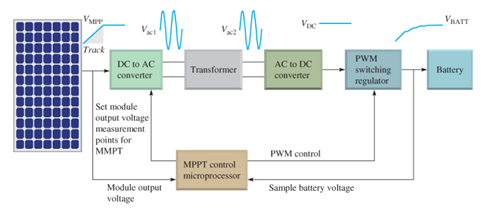
\includegraphics[width=.6\textwidth]{main.png}
    \end{center}
\end{figure}
\section*{Benefits}
A solar panel is consist of several individual cells that are connected in series. This nature increases the internal resistance of the solar panel which makes it inefficient to draw high currents from the panel. With different weather conditions and different times of the day, the panel will give a very fluctuating DC output. It is very important to keep a charge-controlling unit in a solar panel.
\par
One of the key benefits of having our MPPT controller is it can perform well with fluctuating supplies and loading conditions as to charge batteries quickly. Since we hope our solution to be modularized this makes our design to be long-lasting.
\begin{figure}[h]
    \begin{center}
        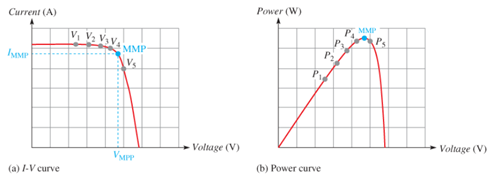
\includegraphics[width=.6\textwidth]{main1.png}
    \end{center}
\end{figure}
\section*{Comparision}
There are many products out in the market that can achieve up to 81\% energy efficiency even in fluctuating weather conditions. But the problem with these solutions is that they are quite expensive to be implemented for low power applications. We expect our design to integrate an analog approach to achieve a low-cost solution.
\section*{Testing \& Demostration}
Although it is not practical to have big solar panels to test and demonstrate our design we hope to buy small solar cells to demonstrate our results in an acceptable manner. In addition to that, we thought of using power supplies as input and providing different loading conditions to demonstrate the performance of our design.
\end{document}
